\documentclass[12pt]{article}
\usepackage{fullpage,enumitem,amsmath,amssymb,graphicx}
\usepackage{listings} % This is a package for including code in your solution.
\usepackage{graphicx} % This is a package for including graphics in your solution.

\title{CS168 Spring Assignment 1}
\author{
	Yueyao Zhu	(yyzhu@stanford.edu) \\
	Yang Du (yd322@stanford.edu)
}

\begin{document}
\maketitle

\section*{Honor Code}

By turning in this assignment, I agree by the Stanford honor code and declare
that all of this is my own work.

\section*{Part 1}

\begin{enumerate}[label=(\alph*)]
 	\item (See code \textbf{simu.py})
 	\item (See \textbf{Figure~\ref{fig:plot}})

Among the four strategies, strategy (a) is simplest in choosing a bin to insert (shortest insertion time), but has the largest number (9 according to the simulation) of balls in the most populated bin. Strategy (b) and (c) lowers the number of balls in the most populated bin to 4, 3 in the simulation, but requires choosing and comparing multiple bins, thus longer insertion time. Strategy (d) has the lowest number of balls in the most populated bin 3, which is the same to Strategy (c), but requires only choosing and comparing 2 bins. Therefore, strategy (d) is the \textbf{sweet spot}, which has a low occupancy of the most populated bin (thus low retrieval time) and reasonable number of bins chosen and compared during insertion (thus low insertion time). Strategy (d) yields the best result if we express the performance as (\# of balls in the most populated bin) * (\# of bins chosen and compared).

	\item 

The strategies of placing balls into bins are analogous to the implementation of hashing with chaining in that:
\begin{enumerate}
	\item Randomly select a bin $\Rightarrow{}$ Perform a universal hashing function
	\item Check the number of balls in a bin $\Rightarrow{}$ Get the length of the linked list of the hash table bucket, i.e. the number of chaining objects in the bucket
	\item Place a ball into a bin $\Rightarrow{}$ Add the object to the linked list of the hash table bucket
\end{enumerate}

Therefore, strategy (a) suggests implementing chaining hashing with one hash function $H$, and storing the object $o$ into the bucket (linked list) $\#H(o)$. Strategy (b), (c) suggest using multiple hash functions $H_1, H_2, ..., H_n$, and storing the object into the one (linked list) with the lowest occupancy (list length) among buckets $\#H_1(o), \#H_2(o), .. \#H_n(o)$, where ties are broken with a random selection. $n=2$ in strategy (b) and $n=3$ in strategy (c).

Strategy (d) suggests having two sets of buckets $B_1$, $B_2$, and use hash functions $H_1:O\rightarrow{}B_1$, $H_2:O\rightarrow{}B_2$ to choose one bucket from each sets. The object is put into the one with fewer objects (shorter linked list) and ties are broken by choosing the one from $B_1$.

The trade-offs exist since a more complex insertion algorithms (using more hash functions and choosing a bucket wisely to lower collision thus the length of each bucket) will increase the insertion time, but lower the number of items in a hash bucket thus may decreasing the search time.

In terms of insertion, Strategy (a) requires only one hash calculation, so as to have the fastest inseration time. Both Strategy (b) and (d) require two hash calculation, and a comparison of the buckets' occupancy. Thus, they have longer insertion time than the strategy (a). Strategy (c) requires three hash calculation and comparations of 3 buckets' occupancy, which makes it the slowest strategy in terms of insertion.

In terms of retrieval, according to the result in part (b), the most populated buckets contain 9 objects for strategy (a), 4 objects for strategy (b), 3 objects for stratety (c), and 3 objects for strategy (d). Thus, strategy (a) may need to check $\approx{}9$ objects, strategy (b) $\approx{}2*4=8$ objects, strategy (c) $\approx{}3*3=9$ objects, and strategy (d) $\approx{}3*2=6$ objects. Therefore, the fourth strategy turn out to be the best while search time is considered.

\end{enumerate}

\begin{figure}[h]
	\centering
	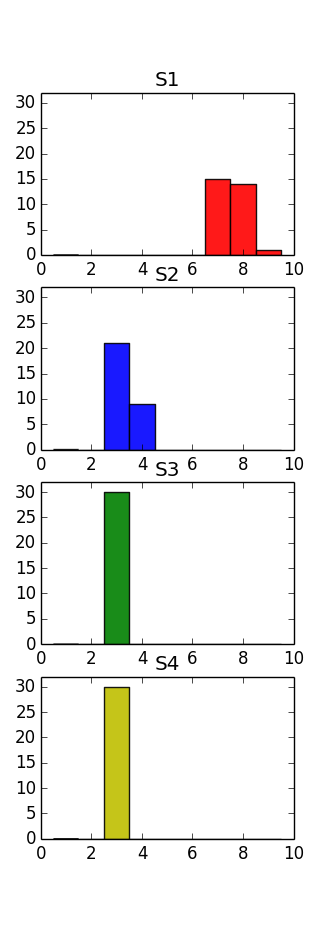
\includegraphics[width=0.4\textwidth]{figure_1.png}
	\caption{Histogram for $X$}
	\label{fig:plot}
\end{figure}

\end{document}